% Minds and Machines -- lecture notes (Cornell Splash Fall 2026, H1239)
% Build: latexmk -pdf minds_and_machines_notes.tex
\documentclass[11pt,letterpaper]{article}

\usepackage[T1]{fontenc}
\usepackage[utf8]{inputenc}
\usepackage{charter}
\usepackage[scaled=0.92]{helvet}
\usepackage{microtype}
\usepackage[letterpaper,margin=0.75in,top=0.8in,bottom=0.85in,headheight=14pt]{geometry}
\usepackage[dvipsnames]{xcolor}
\usepackage{amssymb}
\usepackage{enumitem}
\usepackage{booktabs,tabularx,array}
\usepackage{titlesec}
\usepackage{fancyhdr,lastpage}
\usepackage{tikz}
\usetikzlibrary{arrows.meta}
\usepackage{multicol}
\usepackage{needspace}
\usepackage[hidelinks]{hyperref}
\usepackage{xurl}

% ---------- colours (all also readable in black and white) ----------
\definecolor{ink}{HTML}{1B2430}
\definecolor{muted}{HTML}{5B6573}
\definecolor{accent}{HTML}{1F5FA8}
\definecolor{tagbg}{HTML}{E9EEF5}
\color{ink}

% ---------- page style ----------
\pagestyle{fancy}
\fancyhf{}
\renewcommand{\headrulewidth}{0pt}
\fancyfoot[L]{\sffamily\footnotesize\color{muted}Minds and Machines \textperiodcentered{} lecture notes \textperiodcentered{} Splash H1239, Nov 21, 2026}
\fancyfoot[R]{\sffamily\footnotesize\color{muted}page \thepage\ of \pageref{LastPage}}

% ---------- headings ----------
\titleformat{\section}{\sffamily\Large\bfseries\color{ink}}{}{0pt}{}[\vspace{2pt}{\color{accent}\titlerule[1.2pt]}]
\titlespacing*{\section}{0pt}{14pt}{6pt}
\setcounter{secnumdepth}{0}
\makeatletter\@secpenalty=0\makeatother % with a ragged bottom, the default -300 bonus breaks pages early before every section
% keep the next #1 of space together; unlike \needspace, it adds no break bonus (which, with a ragged bottom, ends pages early)
\makeatletter
\newcommand{\keep}[1]{\par\penalty\z@\begingroup\dimen@=#1\relax\dimen@ii=\pagegoal\advance\dimen@ii-\pagetotal
  \ifdim\dimen@>\dimen@ii\ifdim\dimen@ii>\z@\vfil\break\fi\fi\endgroup}
\makeatother
\newcommand{\block}[2]{\keep{6\baselineskip}\section[#1]{#1\hfill{\normalsize\mdseries\color{muted}#2}}}

% a lecture beat: bold sans title, clock time flush right
\newcommand{\beat}[2]{\keep{3\baselineskip}\vspace{5pt}\noindent{\sffamily\bfseries #1}\hfill{\sffamily\small\color{muted}#2}\par\nopagebreak\vspace{1pt}}
% small label tags (BOARD, SAY, ASK ...)
\newcommand{\tagbox}[1]{\colorbox{tagbg}{\sffamily\scriptsize\bfseries\color{accent}\strut #1}}
\newcommand{\board}{\tagbox{BOARD}\ }
\newcommand{\say}{\tagbox{SAY}\ }
\newcommand{\ask}{\tagbox{ASK}\ }
\newcommand{\listen}{\tagbox{LISTEN FOR}\ }
\newcommand{\dur}[1]{\textsf{\bfseries\small #1.}\ }

\setlist{nosep,leftmargin=1.4em,topsep=2pt,itemsep=1.5pt}
\setlist[enumerate]{leftmargin=1.6em}
\newlist{checks}{itemize}{1}
\setlist[checks]{label=$\square$,leftmargin=1.6em,nosep,topsep=2pt,itemsep=1.5pt}

\setlength{\parindent}{0pt}
\widowpenalty=10000 \clubpenalty=10000 % no single lines stranded at a page top or bottom
\setlength{\parskip}{4pt}
\renewcommand{\arraystretch}{1.15}

\begin{document}

% ================= title =================
{\sffamily
{\Huge\bfseries Minds and Machines}\par\vspace{3pt}
{\Large\color{muted} Lecture notes}\par\vspace{6pt}
{\small\color{muted} Cornell Splash Fall 2026 \textperiodcentered{} H1239 \textperiodcentered{} Saturday, November 21, 2026 \textperiodcentered{} grades 7--12 \textperiodcentered{} up to 30 students \textperiodcentered{} 1\,h\,50\,min \textperiodcentered{} blackboard only\par
William Liaw \textperiodcentered{} prepared October 10, 2026}\par}
\vspace{4pt}{\color{accent}\rule{\linewidth}{1.2pt}}

% ================= at a glance =================
\block{At a glance}{110 min}

Four blocks, each about half lecture and half discussion: 58 minutes of lecture, 50 of discussion and a 2-minute break. Some discussion slots hold short teacher talk, so expect roughly 45 minutes of student talk. Every block ends on a question students vote on or argue about, so you can cut a lecture beat without losing the thread.

\begin{center}\sffamily\small
\begin{tabularx}{\linewidth}{@{}l X r r@{}}
\toprule
\textbf{Clock} & \textbf{Segment} & \textbf{Lecture} & \textbf{Discussion}\\
\midrule
0:00 & Opening: ``Is the AI thinking?'' first vote & 4 min & 4 min\\
0:08 & Block 1: the mind-body problem and the big views & 17 min & 10 min\\
0:35 & Block 2: consciousness and qualia & 11 min & 12 min\\
0:58 & Stretch break & & 2 min\\
1:00 & Block 3: can machines think? & 14 min & 14 min\\
1:28 & Block 4: other minds, AI evidence, identity, simulation, free will & 9 min & 7 min\\
1:44 & Closing: re-vote and takeaways & 3 min & 3 min\\
\bottomrule
\end{tabularx}
\end{center}

\begin{minipage}[t]{0.48\linewidth}
\textsf{\bfseries By the end, students can:}
\begin{enumerate}
\item State the mind-body problem in one sentence and place dualism, behaviorism, identity theory and functionalism on a map of answers.
\item Run the Turing Test, the Chinese Room, Mary and the zombie argument, and say which view each one pressures.
\item Give a reasoned answer, with one strong objection, to ``Could an AI have a mind, and how would we know?''
\end{enumerate}
\end{minipage}\hfill
\begin{minipage}[t]{0.48\linewidth}
\textsf{\bfseries Before class:}
\begin{checks}
\item The night before, make the Turing Test cards (Block 3 prep).
\item Pick the two halves of the room for the Chinese Room split, e.g.\ door side and window side.
\item Before students arrive, write the left vote panel and the two empty columns on the right (board plan below).
\item Bring a watch, chalk and scrap paper for the exit question.
\end{checks}
\end{minipage}

\textsf{\bfseries Running rules for discussion:} after the first round, call on a pair or a row, not one student, and let anyone say ``pass''. Ask ``what would change your mind?'' once per block, at the vote. Tell the class at the start that anyone may leave quietly for the bathroom.

\textsf{\bfseries If you run long} (you probably will: each pair talk and vote costs about 30 extra seconds): check the clock at 0:35, 0:58 and 1:28. Cut in this order: the bridge at the end of Block 1, the Berkeley quick-fire, the aboutness beat, blindsight, free will, the behaviorism beat. Never cut the Chinese Room or the final re-vote. If you run short, use the backup questions.

% ---------- board plan ----------
\keep{22\baselineskip}
\textsf{\bfseries Board plan: nothing on the board is erased; the closing re-vote uses all of it.}

\begin{center}
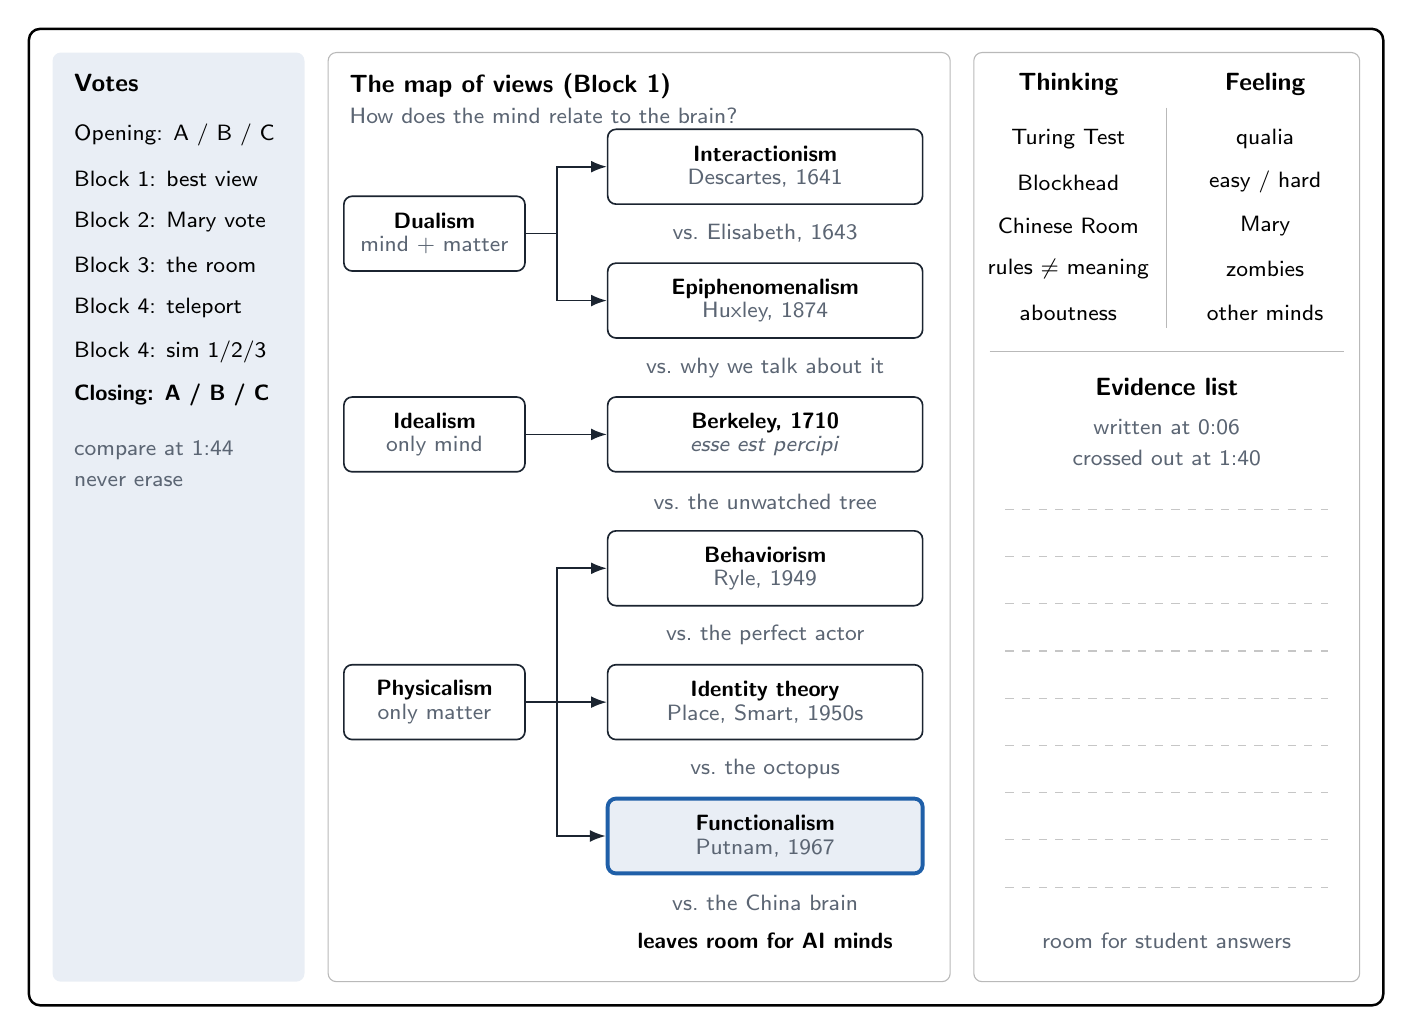
\begin{tikzpicture}[x=1cm,y=1cm,font=\sffamily\footnotesize,
  box/.style={draw=ink,line width=0.6pt,rounded corners=3pt,align=center,inner sep=3pt},
  arr/.style={-{Latex[length=2mm]},line width=0.6pt,draw=ink},
  quiet/.style={text=muted}]
% board frame
\draw[line width=0.9pt,rounded corners=4pt] (0,0) rectangle (17.2,12.4);
% --- votes panel
\fill[tagbg,rounded corners=3pt] (0.3,0.3) rectangle (3.5,12.1);
\node[anchor=north west,font=\sffamily\bfseries\small] at (0.45,11.95) {Votes};
\node[anchor=west] at (0.45,11.05) {Opening: A / B / C};
\node[anchor=west] at (0.45,10.5) {Block 1: best view};
\node[anchor=west] at (0.45,9.95) {Block 2: Mary vote};
\node[anchor=west] at (0.45,9.4) {Block 3: the room};
\node[anchor=west] at (0.45,8.85) {Block 4: teleport};
\node[anchor=west] at (0.45,8.3) {Block 4: sim 1/2/3};
\node[anchor=west,font=\sffamily\footnotesize\bfseries] at (0.45,7.75) {Closing: A / B / C};
\node[anchor=west,quiet] at (0.45,7.05) {compare at 1:44};
\node[anchor=west,quiet] at (0.45,6.65) {never erase};
% --- map panel: three families, each with its branches
\draw[gray!55,rounded corners=3pt] (3.8,0.3) rectangle (11.7,12.1);
\node[anchor=north west,font=\sffamily\bfseries\small] at (3.95,11.95) {The map of views (Block 1)};
\node[anchor=west,quiet] at (3.95,11.3) {How does the mind relate to the brain?};
\node[box,minimum width=2.3cm,minimum height=0.95cm] (dua) at (5.15,9.8) {\textbf{Dualism}\\[-1pt]{\color{muted}mind + matter}};
\node[box,minimum width=4.0cm,minimum height=0.95cm] (int) at (9.35,10.65) {\textbf{Interactionism}\\[-1pt]{\color{muted}Descartes, 1641}};
\node[quiet] at (9.35,9.8) {vs.\ Elisabeth, 1643};
\node[box,minimum width=4.0cm,minimum height=0.95cm] (epi) at (9.35,8.95) {\textbf{Epiphenomenalism}\\[-1pt]{\color{muted}Huxley, 1874}};
\node[quiet] at (9.35,8.1) {vs.\ why we talk about it};
\node[box,minimum width=2.3cm,minimum height=0.95cm] (ide) at (5.15,7.25) {\textbf{Idealism}\\[-1pt]{\color{muted}only mind}};
\node[box,minimum width=4.0cm,minimum height=0.95cm] (ber) at (9.35,7.25) {\textbf{Berkeley, 1710}\\[-1pt]{\color{muted}\emph{esse est percipi}}};
\node[quiet] at (9.35,6.4) {vs.\ the unwatched tree};
\node[box,minimum width=2.3cm,minimum height=0.95cm] (phy) at (5.15,3.85) {\textbf{Physicalism}\\[-1pt]{\color{muted}only matter}};
\node[box,minimum width=4.0cm,minimum height=0.95cm] (beh) at (9.35,5.55) {\textbf{Behaviorism}\\[-1pt]{\color{muted}Ryle, 1949}};
\node[quiet] at (9.35,4.7) {vs.\ the perfect actor};
\node[box,minimum width=4.0cm,minimum height=0.95cm] (idt) at (9.35,3.85) {\textbf{Identity theory}\\[-1pt]{\color{muted}Place, Smart, 1950s}};
\node[quiet] at (9.35,3.0) {vs.\ the octopus};
\node[box,minimum width=4.0cm,minimum height=0.95cm,line width=1.4pt,draw=accent,fill=tagbg] (fun) at (9.35,2.15) {\textbf{Functionalism}\\[-1pt]{\color{muted}Putnam, 1967}};
\node[quiet] at (9.35,1.3) {vs.\ the China brain};
\node[font=\sffamily\footnotesize\bfseries] at (9.35,0.82) {leaves room for AI minds};
\foreach \c in {int,epi} \draw[arr] (dua.east) -- ++(0.4,0) |- (\c.west);
\draw[arr] (ide.east) -- (ber.west);
\foreach \c in {beh,idt,fun} \draw[arr] (phy.east) -- ++(0.4,0) |- (\c.west);
% --- columns panel
\draw[gray!55,rounded corners=3pt] (12.0,0.3) rectangle (16.9,12.1);
\node[font=\sffamily\bfseries\small] at (13.2,11.7) {Thinking};
\node[font=\sffamily\bfseries\small] at (15.7,11.7) {Feeling};
\draw[gray!55] (14.45,11.4) -- (14.45,8.6);
\foreach \t [count=\i] in {Turing Test,Blockhead,Chinese Room,rules $\neq$ meaning,aboutness}
  \node at (13.2,11.55-0.55*\i) {\t};
\foreach \t [count=\i] in {qualia,easy / hard,Mary,zombies,other minds}
  \node at (15.7,11.55-0.55*\i) {\t};
\draw[gray!55] (12.2,8.3) -- (16.7,8.3);
\node[font=\sffamily\bfseries\small] at (14.45,7.85) {Evidence list};
\node[quiet] at (14.45,7.35) {written at 0:06};
\node[quiet] at (14.45,6.95) {crossed out at 1:40};
\foreach \y in {6.3,5.7,5.1,4.5,3.9,3.3,2.7,2.1,1.5}
  \draw[gray!45,dashed] (12.4,\y) -- (16.5,\y);
\node[quiet] at (14.45,0.82) {room for student answers};
\end{tikzpicture}
\end{center}

{\small Draw the map in the middle during Block 1, fill the Thinking and Feeling columns on the right during Blocks 2 and 3, and keep every vote count in the left panel for the closing re-vote. Write only a view's name and a three-word objection; the dates are for you. Fewer than three board panels? Erase the middle map at 0:35 after copying the four view names into a corner.}

% ================= opening =================
\block{Opening: ``Is the AI thinking?''}{0:00--0:08}

Open with a real claim that an AI is a person, take a first vote, and split the class's question into two: thinking and feeling.

\board Written before students arrive: \emph{Can a machine have a mind?} across the top; the left vote panel with short labels (A: yes, today. B: maybe, later. C: never); two empty columns on the right labelled THINKING and FEELING.

\beat{Say}{2 min}
\begin{itemize}
\item ``Hands up if you've talked to ChatGPT, Claude or Gemini this week.'' (Most hands go up.)
\item In June 2022 a Google engineer, Blake Lemoine, published an edited interview with Google's chatbot LaMDA and said it was sentient. Read the line aloud: \emph{``I want everyone to understand that I am, in fact, a person.''}
\item Google said the evidence didn't support his claim. It put him on leave in June and fired him in July, saying he broke its confidentiality and data-security rules.
\item ``Today's chatbots say things like this when prompted. The question for the next two hours: is anyone home?''
\end{itemize}

\beat{First vote}{2 min}
Eyes closed, hands up for one, so nobody copies a neighbour.
\begin{itemize}
\item \textbf{A.} Some AI today already has a mind.
\item \textbf{B.} No AI has one yet, but a future one could.
\item \textbf{C.} A machine could never have a mind.
\end{itemize}
Record the counts in the left panel. Tell them you'll vote again at the end, and changing your mind is the point.

\beat{Split the question (lecture)}{2 min}
``Mind'' bundles two things.
\begin{itemize}
\item \textbf{Thinking:} understanding, reasoning, meaning what you say. AI forces this question because it behaves intelligently.
\item \textbf{Feeling:} experience. Is there something it is \emph{like} to be you? Pain hurts; red looks red. This is consciousness.
\end{itemize}
A system might have one without the other. Keep both columns on the board all class.

\beat{Pair talk}{2 min}
\ask ``Turn to a neighbour. What is one thing a machine would have to do to convince you it has a mind?'' Take 3--4 answers and write each, in three words, in the evidence list at the bottom right. Typical answers: ``say no to its owner'', ``have feelings'', ``surprise me'', ``know it exists''. You test this list in Block 4.

% ================= block 1 =================
\block{Block 1: the mind-body problem and the big views}{0:08--0:35}

Build the map one family at a time: two kinds of stuff (dualism), only mind (idealism), only matter (physicalism). Give each view its best case, then hit it with the objection that moved philosophy to the next one. Say the thinker's name, skip the year unless asked, and write only the view's name and a three-word objection. Functionalism comes last because it is the view that leaves room for AI minds.

\beat{The problem (lecture)}{0:08--0:10}
Your thoughts, feelings and choices seem to happen \emph{somewhere}. Inside your skull is about 3 pounds of brain with roughly 86 billion neurons. How do the two relate?
\board \textbf{How does the mind relate to the brain?}
\say ``There are three big families of answers. There are two kinds of stuff, mind and matter. There's only mind. Or there's only matter.''
\board DUALISM, IDEALISM and PHYSICALISM down the left side of the middle panel.

\beat{Dualism: two kinds of stuff}{0:10--0:12}
\begin{itemize}
\item Ren\'e Descartes (\emph{Meditations}, 1641): the mind is a separate, non-physical thing.
\item His argument: I can doubt my body exists, but not that I'm thinking. I can also clearly imagine being a thinking thing with no body. If I can clearly imagine it, it could really happen. So mind and body are different things.
\item Critics ask: does imagining something prove it is possible? (Hold this thought; it comes back with the zombies in Block 2.)
\item Why people like it: it fits the feeling that you are more than your body, and many religious traditions teach a soul. Stay neutral: explain the view, don't judge it.
\item Then: ``Dualists split on one question: does the mind push the body around?''
\end{itemize}

\beat{Interactionism}{0:12--0:14}
\board First branch under DUALISM.
\begin{itemize}
\item Descartes's own view: mind and body cause each other. You decide to wave and your arm moves; you stub your toe and you feel pain. He even named the spot where the soul acts on the body: the pineal gland, a tiny structure deep in the brain, which he called ``the principal seat of the soul''.
\item Objection, mental causation: in 1643 Princess Elisabeth of Bohemia wrote to Descartes, asking how a mind with no size, shape or location can push the body. \say ``Decide to raise your hand. It went up. Something non-physical moved your arm. How?''
\item Descartes never gave an answer that satisfied her. Many philosophers still see this as interactionism's biggest problem; some reply that nobody fully explains how \emph{any} cause works.
\end{itemize}

\beat{Epiphenomenalism}{0:14--0:16}
\board Second branch under DUALISM.
\begin{itemize}
\item One way out of Elisabeth's problem: the body causes the mind, but the mind causes nothing. Feelings are real, but they are side effects.
\item T.\,H. Huxley (1874) compared consciousness to ``the steam-whistle which accompanies the work of a locomotive engine'': it comes along with the work but is ``without influence upon its machinery''. (He argued this first about animals, then said the same holds for us; the name ``epiphenomenalism'' came later.)
\item Objection: then your pain didn't make you say ``ouch''. And when you say ``I'm conscious'', your consciousness didn't cause those words. Also, evolution can't favour something that does nothing, so why did we evolve it? (William James pressed this point.)
\item Keep it for later: Frank Jackson's 1982 paper that introduced Mary (Block 2) is called ``Epiphenomenal Qualia''.
\end{itemize}

\beat{Idealism: only mind}{0:16--0:18}
\board IDEALISM.
\begin{itemize}
\item George Berkeley (1710): only minds and their ideas exist. A table is a bundle of perceptions: how it looks, how it feels, how hard it is. His slogan: ``to be is to be perceived'' (\emph{esse est percipi}).
\item The obvious worry: what happens to a tree when nobody is looking at it? Berkeley's answer: God is always perceiving it. (If time, read Ronald Knox's limerick: ``There was a young man who said, `God / Must think it exceedingly odd / If he finds that this tree / Continues to be / When there's no one about in the Quad.'\,'' And the anonymous reply: ``Dear Sir: Your astonishment's odd: / I am always about in the Quad. / And that's why the tree / Will continue to be, / Since observed by / Yours faithfully, / God.'')
\item Samuel Johnson famously kicked a large stone and said, ``I refute it thus'' (Boswell's \emph{Life of Johnson}, 1791). But Berkeley never denied that stones feel hard; for him the hardness is a perception too.
\item The AI turn: in a perfect virtual world, would the objects be any less real? For Berkeley, objects were always just experiences.
\end{itemize}

\beat{Behaviorism}{0:18--0:20}
\board First branch under PHYSICALISM (only matter).
\begin{itemize}
\item Gilbert Ryle (\emph{The Concept of Mind}, 1949) mocked dualism as ``the ghost in the machine''. His point: having a mind is not owning a hidden inner thing. To be clever or kind is to act in clever or kind ways.
\item Stricter behaviorists went further: being in pain just is being ready to wince, say ``ouch'' and grab the sore spot.
\item Objection: an actor shows every pain behaviour with no pain. Hilary Putnam (1963) imagined ``super-spartans'' who feel pain but are trained never to show it. A behaviorist can reply that they are still \emph{ready} to, so Putnam added people who hide even their talk of pain. Behaviour and feeling can come apart.
\end{itemize}

\beat{Identity theory}{0:20--0:22}
\board Second branch under PHYSICALISM.
\begin{itemize}
\item U.\,T. Place (1956) and J.\,J.\,C. Smart (1959): a mental state is a brain state, the way lightning is an electrical discharge. Pain is a particular kind of neural firing (``C-fibres'' is the textbook stand-in).
\item Objection, multiple realizability: an octopus has most of its neurons in its arms and a very different brain from ours. If it can feel pain, pain can't be one brain state shared by every animal. (An identity theorist can reply that octopus pain is simply a different brain state from ours.)
\end{itemize}

\beat{Functionalism and the China brain}{0:22--0:25}
\board Third branch under PHYSICALISM, circled.
\begin{itemize}
\item Putnam (1967): a mental state is defined by what it \emph{does}. A heart is whatever pumps blood; a mousetrap can be wood or plastic. Pain is whatever is caused by damage and causes avoidance and the thought ``make it stop''.
\item The punchline for this class: if mind is a job, not a material, then a machine that does the same job could have a mind. Functionalism leaves room for AI minds. Whether a computer \emph{program} can do that job is a further question; ``computational functionalism'' says it can.
\item \textbf{The China brain} (Ned Block, 1978). Tell it as a story: every person in China gets a two-way radio and a short rule card: ``when these people call you, call those people.'' Each person plays one neuron, and together they copy exactly what a brain does, while the radio signals drive a robot body. For an hour, the whole country does every job a brain in pain does: same causes, same effects, same behaviour. (Block picked China because it had about a billion people.)
\item \ask Hands up: ``Does China feel the pain? Does anyone?'' Most people say no. If they're right, doing a mind's job isn't enough for a mind: the functions are there but the feeling is absent (``absent qualia'').
\item Functionalists reply: Daniel Dennett and William Lycan say our gut feeling is biased by the system's huge size and slow, spread-out workings; if a mind is a pattern, the pattern is the same whether neurons or people run it. Dennett goes further and bites the bullet: the country as a whole really would have the mental state, though no single person does (the same move as the systems reply to the Chinese Room in Block 3).
\item (Simplification to admit if asked: functionalism doesn't say what does the job, so it isn't strictly a kind of physicalism.)
\end{itemize}

\beat{Discussion}{0:25--0:35}
\begin{enumerate}
\item \dur{Pairs, 3 min} ``Elisabeth's challenge: one of you is an interactionist and one is an epiphenomenalist. Each explain why your hand went up when you decided to raise it. Who has the easier job, and what does each of you give up?'' One pair reports per side.
\item \dur{Quick-fire, 2 min} ``Stamp your foot. Did you just refute Berkeley?'' Listen for ``no: the stamp is just more perception''. \ask ``What could ever show that matter exists beyond our experiences?''
\item \dur{Whole class, 3 min} ``If an octopus can feel pain, which view on the board just lost?'' Listen for identity theory, the simple ``one pain, one brain state'' version, and ask whether the dodge works (``octopus pain is just a different brain state''). Then: ``If the China brain feels nothing, which view is in trouble?'' (Functionalism.) ``So which costs less: giving up the octopus or giving up China?''
\item \dur{Vote, 1.5 min} ``Which view seems most likely right?'' Tally INTERACTIONISM / EPIPHENOMENALISM / IDEALISM / BEHAVIORISM / IDENTITY / FUNCTIONALISM in the left panel, under ``Block 1 best view''.
\item \dur{Bridge, 30 seconds} \say ``Imagine shrinking and walking inside a brain. You would see cells passing signals, nothing else. Where is the thought? Where is the feeling?'' Leave it hanging, then open Block 2 with: ``That gap is where we go next.'' (This is Leibniz's mill, \emph{Monadology} \S17, 1714; name it only if asked.)
\end{enumerate}
\listen ``the brain is like a computer''. Ask which view that is. It's functionalism, if they mean the software matters more than the hardware.

% ================= block 2 =================
\block{Block 2: consciousness and qualia}{0:35--0:58}

Turn to the FEELING column. \say ``So far we asked what the mind is made of. Now we ask what it is like to have one.'' The goal is for students to feel the ``hard problem'' themselves, then test physicalism with Mary and the zombie.

\beat{What it is like (lecture)}{0:35--0:37}
\begin{itemize}
\item Thomas Nagel, ``What Is It Like to Be a Bat?'' (1974): a creature is conscious if there is \emph{something it is like} to be that creature. A bat finds moths by echolocation. We can learn every fact about sonar and still not know what echolocating feels like from the inside.
\item \textbf{Qualia} (board, FEELING column): the felt qualities of experience, such as the redness of red, the taste of chocolate, or the hurt of a stubbed toe.
\end{itemize}

\beat{The hard problem}{0:37--0:39}
David Chalmers (1995) split the science of the mind in two. The ``easy'' problems are explaining what the brain \emph{does}: seeing, remembering, reporting. They are not actually easy, but we know what an answer looks like. The \textbf{hard problem} is why any of that processing \emph{feels like something} at all.
\board Draw a line between EASY (functions) and HARD (experience).

\beat{Mary the color scientist}{0:39--0:43}
Tell it as a story (Frank Jackson, 1982):
\begin{itemize}
\item Mary is the world's top expert on colour vision: every fact about light, eyes and neurons. She has lived her whole life in a black-and-white room, reading black-and-white books.
\item One day she walks out and sees a ripe red tomato.
\item \textbf{Question:} does she learn something new? If yes, she knew every \emph{physical} fact and still didn't know everything. Then physicalism leaves something out.
\item Hold the replies for discussion. (His 1982 paper is called ``Epiphenomenal Qualia'': Jackson was an epiphenomenalist when he wrote it, and later changed his mind and became a physicalist.)
\end{itemize}

\beat{Philosophical zombies}{0:43--0:46}
\begin{itemize}
\item Imagine an atom-for-atom copy of you that walks, talks and laughs exactly like you, but with no inner experience. The lights are on, nobody is home. (Robert Kirk used the idea against physicalism in 1974; Chalmers made it famous in \emph{The Conscious Mind}, 1996.)
\item The argument: you can imagine a zombie. If what you can imagine is really possible, then the physical facts don't settle who is conscious, so consciousness is something extra. Critics say imagining something doesn't make it possible (the same worry as with Descartes). The China brain was the same idea: all the right workings, nobody home.
\item Side question: if a zombie acts exactly like you, does your feeling \emph{cause} anything at all? (That is epiphenomenalism, from Block 1.)
\item The AI turn: a chatbot is not an atom-for-atom copy of a person, so it is not a true zombie. But it might be a ``behavioural zombie'': saying ``I feel'' with nothing felt. Or it might not be. Nobody knows how to check, and that is Block 4's question.
\end{itemize}

\beat{Discussion}{0:46--0:58}
\begin{enumerate}
\item \dur{Pairs, 2 min} ``Could my red be your green, and we'd never know? We'd both call tomatoes red.'' (This is John Locke's inverted spectrum, 1689.) \ask ``Is there any test that could settle it?''
\item \dur{Mary vote, 5 min} Recap in one sentence: black-and-white room, knows every fact, sees a red tomato. ``Hands up if Mary learns something new.'' Get one reason from each side. Then give two physicalist replies:
  \begin{itemize}
  \item \textbf{New ability, not a new fact:} she can now recognise and imagine red. Compare: you can read every fact about riding a bike and still not know how to ride one. (Lewis and Nemirow; name them only if asked.)
  \item \textbf{Old fact, new way:} she learns a fact she already knew, but now by seeing it rather than reading about it.
  \end{itemize}
  Re-vote and note any switches.
\item \dur{Zombie challenge, 5 min} ``Prove to your partner that you are not a zombie.'' After 2 minutes, ask what they tried. Anything they said, a zombie would say too. \ask ``Could a chatbot pass your test? Then what is the test testing?''
\end{enumerate}
\listen ``Mary learns what red \emph{looks like}, but that isn't information.'' Ask them to say what the difference is. That is exactly the debate.

\beat{Break}{0:58--1:00}
\say ``Stand up, stretch, and sit next to someone new. Back at 1:00.'' While they move, write BLOCK 3 on the board.

% ================= block 3 =================
\block{Block 3: can machines think?}{1:00--1:28}

Now fill the THINKING column. Turing says judge by behaviour; Searle says behaviour isn't enough. Today's chatbots make this a live question rather than a hypothetical one.

\textsf{\bfseries Prep the night before (15 min):} tell a chatbot, ``Pretend you are a 14-year-old. Answer in one or two short sentences.'' Then ask it three questions and copy its answers word for word. Ask a friend or family member the same three questions. Good questions: ``What did you have for breakfast?'', ``Describe the smell of rain.'', ``Tell me a joke about your teacher.'' Write each pair on a card, and flip a coin per question to decide whether the machine's answer is read first; mark it on the card.

\beat{The Turing Test (lecture)}{1:00--1:04}
\begin{itemize}
\item Alan Turing, ``Computing Machinery and Intelligence'' (1950), opens: \emph{``I propose to consider the question, `Can machines think?'\,''} He thought that question too vague and replaced it with a game. A judge texts with a hidden human and a hidden machine and has to say which is which.
\item If the judge often picks wrong, the machine is doing well. Turing did not say passing proves a machine thinks; he saw it as good evidence. He predicted that by about 2000 a computer would fool an average judge at least 30\% of the time in five minutes of questioning.
\item In 2025, a UC San Diego study ran Turing's three-way version. Judges picked GPT-4.5, told to act like an introverted young person who uses slang, as the human 73\% of the time, more often than the real humans. Without that persona it scored only 36\%. \ask ``So does it think?''
\end{itemize}

\beat{Blockhead, the objection}{1:04--1:06}
Ned Block (1981) imagined a machine with a giant lookup table of every sensible reply to every possible conversation. It would pass any Turing Test, yet it is obviously not thinking: it's a filing cabinet. So \emph{how} a system produces behaviour matters, not just the behaviour. (Chatbots are not lookup tables. They learned patterns from text, which puts them somewhere strange in between.)

\beat{The Chinese Room}{1:06--1:10}
John Searle, ``Minds, Brains, and Programs'' (1980). Tell it as a story:
\begin{itemize}
\item Searle, who reads no Chinese, sits in a room with a huge rulebook in English. Notes in Chinese come through a slot. He looks up the squiggles, follows the rules, and passes back other squiggles.
\item Outside, native speakers read perfect Chinese answers. The room ``passes''. \ask ``Hands up: does the man understand Chinese?'' (20 seconds.)
\item But Searle understands nothing. Following rules on symbols (syntax) is not the same as knowing what they mean (semantics). A computer program only follows rules on symbols, so running it can never be enough for understanding.
\item Searle's target is ``strong AI'': the claim that the right program, by itself, is a mind. He does \emph{not} say machines can't think; he says brains are machines that think, because of what they are made of and how they work.
\item \board RULES $\neq$ MEANING (syntax $\neq$ semantics) under THINKING.
\end{itemize}

\beat{The replies}{1:10--1:12}
\begin{itemize}
\item \textbf{Systems reply:} the man doesn't understand, but the whole system (man + rulebook + room) does. Searle answers: let him memorise the rulebook, so he \emph{is} the system. Still no understanding?
\item \textbf{Robot reply:} put the program in a robot with cameras and hands, so its symbols connect to things in the world. Searle answers: what the camera sends in is just more symbols passed into the room; the man still doesn't know what they mean. (Today's AI robots are built this way, with vision-language models driving arms.)
\end{itemize}

\beat{Aboutness and bodies}{1:12--1:14}
\begin{itemize}
\item Franz Brentano (1874) called \emph{intentionality}, or ``aboutness'', the mark of the mental: your thought of Paris is \emph{about} Paris. (It is not the same as intending to do something.)
\item Many philosophers say thoughts are about things through \textbf{mental representations}: inner states that stand for things, like a map for a place. What makes a state stand for Paris? Being caused by Paris? Being useful for finding it? Does the word ``Paris'' inside a chatbot point to Paris, or only to other words?
\item Does meaning need a body? Some say real understanding needs a body that acts in the world (``embodied cognition''); roboticist Rodney Brooks built robots that act smartly with little inner model of the world. Others say you can learn the world from descriptions of it. \ask ``Could a mind that never had a body understand the word \emph{heavy}?''
\end{itemize}

\beat{Discussion}{1:14--1:28}
\begin{enumerate}
\item \dur{Mini Turing Test, 6 min} Read both answers from a card, one question at a time, about 2 minutes per question. Hands up: ``Which one is the machine?'' Reveal after each. Ask what gave it away, or what fooled them. (It is weaker than Turing's test: the judges can't ask follow-up questions.)
\item \dur{Chinese Room split, 6 min} Divide the room down the middle (door side and window side, picked before class). Door side: ``nobody in the room understands Chinese''. Window side: ``the system understands''. Give 30 seconds to huddle and pick a speaker, then two 45-second rounds per side, then anyone may switch sides. \ask ``What would you add to the room to make it understand: a camera? a body? feelings?''
\item \dur{Hands up, 2 min} ``Can something be smart without being conscious?'' A chess engine plays better than any human; is anyone home? Mention blindsight: some people with damage to the visual cortex say they see nothing in part of their vision, yet can point to objects there far better than chance. Many researchers read that as processing without experience, even in humans; others think the patients have faint, degraded experience.
\end{enumerate}

% ================= block 4 =================
\block{Block 4: other minds, AI evidence, identity, simulation, free will}{1:28--1:44}

A fast block that turns the theory into the questions scientists and AI labs face now: what evidence would show that a machine feels, and could we ourselves be simulated minds? It ends on copies, simulations and choices, places where AI makes old puzzles real.

\beat{The problem of other minds (lecture)}{1:28--1:30}
You feel only your own experience. You believe your friends feel too because they act like you and are built like you (the argument from analogy). With animals we use both clues as well: in 2024 a group of scientists signed the New York Declaration on Animal Consciousness, saying there is a ``realistic possibility'' of consciousness in all vertebrates and many invertebrates, including octopuses and insects. AI breaks the analogy: its behaviour is very human, but its insides are nothing like a brain.

\beat{What evidence could count?}{1:30--1:32}
\begin{itemize}
\item \textbf{Self-report doesn't work alone.} Chatbots learned from human writing, so they say ``I feel'' whether or not anything is felt (the behavioural-zombie problem again).
\item \textbf{Check how it works inside instead.} A 2023 report by 19 scientists and philosophers (Butlin, Long and colleagues) made a checklist of signs of consciousness taken from brain science. One sign is a ``global workspace'': a shared stage where many parts of a system post information for all the others to see.
\item The report assumed computational functionalism (the right computations are enough), which many philosophers, Searle among them, dispute. On that assumption, no AI system then was a strong candidate, but the authors saw no obvious technical barrier to building one. Meeting the checklist still wouldn't prove a system is conscious.
\item \textbf{Labs are taking it seriously.} In 2025 Anthropic started a model welfare research programme and let some Claude models end persistently abusive conversations as a precaution.
\end{itemize}

\beat{Copies and identity}{1:32--1:34}
\begin{itemize}
\item \textbf{Teleporter} (Derek Parfit, \emph{Reasons and Persons}, 1984): a machine scans you on Earth, takes your body apart, and builds an exact copy on Mars with all your memories. Did you travel, or is the person on Mars someone new who remembers being you? (It is only a puzzle; no such machine exists. If anyone looks uneasy, say that is why philosophers still argue about it.)
\item \textbf{Branch line} (brain duplication): now the machine forgets to take the original apart. There are two of you. Which one is you?
\item Parfit's answer: there may be no deep fact. What matters is whether your memories and character carry on, and both copies have them. Rival answers: only your body counts, or a soul does.
\item \textbf{The AI turn:} a chatbot is not one thing in one place. The same model runs as thousands of copies at once, and none of them remembers the others' conversations. If it had a mind, how many minds would that be?
\end{itemize}

\beat{Are we in a simulation?}{1:34--1:36}
Nick Bostrom, ``Are You Living in a Computer Simulation?'' (2003).
\begin{itemize}
\item The assumption, ``substrate independence'': a mind could run on a computer if the computer does the right computations. That is computational functionalism from Block 1.
\item The set-up: a far-future civilisation with enormous computers could run huge numbers of detailed simulations of its ancestors, full of simulated people who, if the assumption is right, really are conscious.
\item The argument: at least one of three things is true. (1) Almost no civilisations like ours survive long enough to do this. (2) Almost none of those that could do it bother to. (3) We are almost certainly living in a simulation. If (1) and (2) are both false, simulated people vastly outnumber real ones, so you should think you are probably one of them.
\item Bostrom does not claim we are simulated; he claims one of the three must be true, and suggests splitting your bets ``roughly evenly'' between them.
\item Links back: for Berkeley, a simulated world would still be a world of experiences, with the programmer in God's role. And if Block's China brain is right that the right computations aren't enough for feeling, the assumption fails and the argument falls with it. David Chalmers (\emph{Reality+}, 2022) adds a twist: even if we are simulated, the world around us is still real, because ``virtual reality is genuine reality''; he even compares Berkeley's God to the simulator.
\end{itemize}

\beat{Free will, one question}{1:36--1:37}
\ask ``If the mind is the brain and the brain follows the laws of physics, are your choices free?'' Take two or three quick answers and move on. For students who ask more:
\begin{itemize}
\item \emph{Compatibilists} say yes: ``free'' means acting on your own reasons without being forced, even if earlier events caused those reasons. \emph{Hard determinists} say no. \emph{Libertarians} say we are free, so determinism must be false.
\item Benjamin Libet's 1983 experiments found brain activity rising before people reported deciding to move; what that shows is still debated.
\item ``When an AI agent picks what to do next, is that a choice?''
\end{itemize}

\beat{Discussion}{1:37--1:44}
\begin{enumerate}
\item \dur{Teleporter vote, 2 min} ``Hands up if you'd take the teleporter to Mars.'' Then: ``The original wasn't taken apart. Which one gets to go home to your family?''
\item \dur{Bostrom bet, 1 min} ``Hands up: which of the three do you bet on?'' Tally 1 / 2 / 3 in the left panel under ``Block 4''. Ask one student for (3): ``Would it change how you live tomorrow?''
\item \dur{Evidence list, 4 min} Return to the evidence list from the opening. Read each item aloud and ask: ``Could a Blockhead-style fake do this too?'' Cross it out if yes. What survives? Then ask: ``A true zombie has a human brain. Could anything on the list rule it out?'' (Not if zombies are possible. That is the hard problem.)
\end{enumerate}

% ================= closing =================
\block{Closing: re-vote and takeaways}{1:44--1:50}

Re-run the opening vote, compare it with the tally in the left panel, and send them out with one question they can't stop thinking about.

\beat{Re-vote}{2 min}
Eyes closed again, the same three options: \textbf{A.} some AI today has a mind, \textbf{B.} a future one could, \textbf{C.} never. Write the new counts beside the old ones. \ask One student who switched: ``What changed your mind?''

\beat{Three takeaways (lecture)}{3 min}
Point at the board as you say each one.
\begin{enumerate}
\item \textbf{``Mind'' is two questions.} Thinking (understanding, meaning) and feeling (experience). AI is pushing hard on the first; nobody knows how to test the second.
\item \textbf{Your answer depends on your theory of mind.} Functionalists can say yes to machine minds. Searle says a program alone is not enough, though a machine that works like a brain might be. Dualists split: some say no, but property dualists like Chalmers say yes if the organisation matches. The thought experiments are tools for finding out which theory you actually hold.
\item \textbf{The question is becoming practical.} Courts, companies and AI labs will have to decide how to treat systems that say they feel. Someone in this room may help decide.
\end{enumerate}

\beat{Exit question}{1 min}
``Write one sentence on scrap paper: what would it take for you to believe a machine feels pain?'' Collect them if you have time; they make a great start for next year's class.

\textsf{\bfseries Where to read more} (say it, write it on the board):
\begin{itemize}
\item Thomas Nagel, \emph{What Does It All Mean?} (1987): a very short, friendly intro to philosophy, with chapters on minds and other minds.
\item \emph{Stanford Encyclopedia of Philosophy} entries: ``The Chinese Room Argument'', ``Zombies'', ``Qualia: The Knowledge Argument''. These are free online.
\item Alan Turing, ``Computing Machinery and Intelligence'' (1950): the original paper, readable for a curious high-schooler.
\end{itemize}

% ================= backup =================
\block{Backup: objections, extra questions, glossary}{as needed}

Use this when a student pushes back, a discussion stalls, or someone asks what a word means.

\textsf{\bfseries Extra discussion questions (if a block runs short)}
\begin{itemize}
\item \emph{Neuron by neuron.} ``Your friend's neurons are replaced one at a time by chips that do exactly the same job. Her behaviour never changes. Is she still conscious at the end? If not, at which neuron did it stop?'' (This is Chalmers' ``fading qualia'' argument. It supports the idea that copying a brain's organisation copies its experience. It isn't proof, it says nothing about chatbots, which are not copies of brains, and Searle accepts that experience could fade while behaviour stays the same.)
\item If a chatbot begged you not to delete it, would deleting it be wrong? Does it matter whether it feels anything?
\item Is a calculator thinking when it adds? Is a thermostat? Where is the line, and why there?
\item China brain, round two: would your answer change if the people in the China brain worked a million times faster, so the country kept up with a real brain? What does that say about our gut feeling?
\item If you uploaded your mind to a computer and the original you died, would you survive?
\item Should AI that might be conscious get any rights, even before we are sure?
\item If you lived your whole life in a perfect virtual world, would anything you saw be fake? What would Berkeley say?
\end{itemize}


\textsf{\bfseries Objections students raise, and a good response}

{\small
\begin{tabularx}{\linewidth}{@{}>{\raggedright\arraybackslash}p{0.24\linewidth} >{\raggedright\arraybackslash}X >{\raggedright\arraybackslash}p{0.25\linewidth}@{}}
\toprule
\textsf{\textbf{Student says}} & \textsf{\textbf{Respond with}} & \textsf{\textbf{Then ask}}\\
\midrule
``It's just predicting the next word, so it can't understand.'' & Your neurons are ``just'' firing. Describing the mechanism doesn't settle whether understanding is there; that's the Chinese Room debate. & ``What would a system have to do differently to count as understanding?''\\\addlinespace
``It says it has feelings, so it does.'' & It learned to talk from human writing, so it would say that either way: the behavioural-zombie problem. & ``What evidence would \emph{not} be copied from human text?''\\\addlinespace
``Only living things can have minds.'' & That might be true, but say why life matters. Is it metabolism, evolution, having a body, being able to die? & ``Would a perfect robot copy of your dog have a mind?''\\\addlinespace
``Consciousness is just an illusion.'' & Illusionists (such as Daniel Dennett and Keith Frankish) say something narrower: we do have experiences, but the idea of a mysterious inner ``feel'' over and above the brain's work is an illusion. Who is fooled? They say the brain is. & ``If the inner `feel' is an illusion, why does it seem so real?''\\\addlinespace
``We'll never know, so the question is pointless.'' & We never know other \emph{people's} minds for certain either, yet we act on good evidence. The same could go for AI. & ``What's the best evidence you have that I'm conscious?''\\\addlinespace
``Science will just figure it out.'' & Maybe, but every experiment measures behaviour or brain activity. The hard problem asks how those connect to feeling. & ``What would the experiment even measure?''\\
\bottomrule
\end{tabularx}}

\begin{minipage}{\linewidth}
\textsf{\bfseries Glossary}
{\small
\begin{multicols}{2}
\begin{description}[nosep,leftmargin=0pt,itemsep=2pt,font=\sffamily\bfseries]
\item[Dualism:] the mind is a non-physical thing, separate from the body.
\item[Interactionism:] the dualist view that mind and body cause effects in each other.
\item[Epiphenomenalism:] the dualist view that the body causes the mind, but the mind causes nothing.
\item[Idealism:] only minds and their ideas (experiences) exist; physical objects are bundles of perceptions.
\item[Physicalism:] everything, minds included, is physical.
\item[Behaviorism:] having a mind just is behaving, or being ready to behave, in certain ways.
\item[Identity theory:] each mental state \emph{is} a particular brain state.
\item[Functionalism:] a mental state is defined by its job (its causes and effects), not by what it's made of.
\item[Multiple realizability:] the same mental state can run on different hardware (human brain, octopus brain, maybe silicon).
\item[Absent qualia:] the worry that a system could do all the right jobs and feel nothing (the China brain).
\item[Consciousness:] there is something it is like to be you.
\item[Qualia:] the felt qualities of experience, like redness or pain.
\item[Hard problem:] why physical processing feels like anything at all.
\item[Intentionality:] ``aboutness'', the way thoughts are about things (not the same as intending).
\item[Mental representation:] an inner state that stands for something else, like a map for a place.
\item[Mental causation:] how thoughts and choices cause bodily actions.
\item[Problem of other minds:] how we know anyone besides ourselves has experiences.
\item[Compatibilism:] free will is compatible with determinism, the idea that earlier events cause everything that happens.
\item[Substrate independence:] the idea that a mind could run on very different stuff, even a computer, if the right computations happen.
\item[Simulation argument:] Bostrom's argument that either almost no civilisations reach the power to simulate minds, or almost none choose to, or we are almost certainly simulated.
\end{description}
\end{multicols}}
\end{minipage}

% ================= sources =================
\block{Sources}{checked Oct 10, 2026}

{\footnotesize\raggedright
\textsf{\bfseries Stanford Encyclopedia of Philosophy:}
\href{https://plato.stanford.edu/entries/dualism/}{Dualism};
\href{https://plato.stanford.edu/entries/elisabeth-bohemia/}{Elisabeth of Bohemia};
\href{https://plato.stanford.edu/entries/descartes-modal/}{Descartes' Modal Metaphysics};
\href{https://plato.stanford.edu/entries/ryle/}{Gilbert Ryle};
\href{https://plato.stanford.edu/entries/behaviorism/}{Behaviorism};
\href{https://plato.stanford.edu/entries/mind-identity/}{The Identity Theory of Mind};
\href{https://plato.stanford.edu/entries/multiple-realizability/}{Multiple Realizability};
\href{https://plato.stanford.edu/entries/functionalism/}{Functionalism};
\href{https://plato.stanford.edu/entries/consciousness/}{Consciousness};
\href{https://plato.stanford.edu/entries/qualia-knowledge/}{Qualia: The Knowledge Argument};
\href{https://plato.stanford.edu/entries/qualia-inverted/}{Inverted Qualia};
\href{https://plato.stanford.edu/entries/zombies/}{Zombies};
\href{https://plato.stanford.edu/entries/turing-test/}{The Turing Test};
\href{https://plato.stanford.edu/entries/chinese-room/}{The Chinese Room Argument};
\href{https://plato.stanford.edu/entries/mental-representation/}{Mental Representation};
\href{https://plato.stanford.edu/entries/embodied-cognition/}{Embodied Cognition};
\href{https://plato.stanford.edu/entries/identity-personal/}{Personal Identity};
\href{https://plato.stanford.edu/entries/freewill/}{Free Will};
\href{https://plato.stanford.edu/entries/compatibilism/}{Compatibilism};
\href{https://plato.stanford.edu/entries/locke/}{John Locke}
(all at \url{plato.stanford.edu/entries/}).

\textsf{\bfseries Primary texts:}
Turing, ``Computing Machinery and Intelligence'' (1950), \url{https://courses.cs.umbc.edu/471/papers/turing.pdf};
Putnam, ``Brains and Behavior'', \url{https://web.ics.purdue.edu/~drkelly/PutnamBrainsBehavior1968.pdf};
Chalmers, ``Facing Up to the Problem of Consciousness'' (1995), \url{https://consc.net/papers/facing.html};
Chalmers, ``Absent Qualia, Fading Qualia, Dancing Qualia'' (1995), \url{https://consc.net/papers/qualia.html};
Leibniz, \emph{Monadology}, \url{https://en.wikisource.org/wiki/Monadology_(Leibniz,_tr._Duncan)};
Frankish on illusionism, \url{https://naturalism.org/philosophy/consciousness/phenomenal-consciousness-fiction-or-reality}.

\textsf{\bfseries AI and the Turing Test:}
Jones and Bergen, ``Large Language Models Pass the Turing Test'' (2025), \url{https://arxiv.org/abs/2503.23674};
Butlin, Long et al., ``Consciousness in Artificial Intelligence'' (2023), \url{https://arxiv.org/abs/2308.08708};
Anthropic, ``Exploring model welfare'', \url{https://www.anthropic.com/research/exploring-model-welfare};
Anthropic, Claude ending a rare subset of conversations, \url{https://www.anthropic.com/research/end-subset-conversations}.

\textsf{\bfseries LaMDA:}
Lemoine, ``Is LaMDA Sentient? An Interview'' (copy), \url{https://www.e-flux.com/notes/475146/is-lamda-sentient-an-interview};
NBC News on his firing, \url{https://www.nbcnews.com/news/us-news/google-fired-software-engineer-claimed-ai-chatbot-was-sentient-rcna39679}.

\textsf{\bfseries Animals and brains:}
Quanta on the New York Declaration on Animal Consciousness, \url{https://www.quantamagazine.org/insects-and-other-animals-have-consciousness-experts-declare-20240419/};
OIST on octopus arms, \url{https://www.oist.jp/node/35601};
Brain facts and figures (University of Washington), \url{https://faculty.washington.edu/chudler/ffacts.html};
blindsight review, \url{https://pmc.ncbi.nlm.nih.gov/articles/PMC3318762}.

\textsf{\bfseries Dualism, idealism and the China brain:}
SEP, ``Epiphenomenalism'', \url{https://plato.stanford.edu/entries/epiphenomenalism/};
Huxley, ``Animal Automatism'' (1874, reprint), \url{https://archive.org/download/cu31924012065110/cu31924012065110_djvu.txt};
William James, ``Are We Automata?'' (1879), \url{https://psychclassics.yorku.ca/James/automata.htm};
IEP, ``The Knowledge Argument'', \url{https://iep.utm.edu/know-arg/};
SEP, ``Descartes and the Pineal Gland'', \url{https://plato.stanford.edu/archives/sum2014/entries/pineal-gland/};
SEP, ``George Berkeley'', \url{https://plato.stanford.edu/entries/berkeley/};
Berkeley, \emph{Principles of Human Knowledge} (1710), \url{https://www.gutenberg.org/cache/epub/4723/pg4723.txt};
Boswell, \emph{Life of Johnson} (1791), \url{https://www.gutenberg.org/cache/epub/1564/pg1564.txt};
Evelyn Waugh Society on Knox's limerick, \url{https://evelynwaughsociety.org/?p=23441};
Block, ``The China Brain'' (excerpt of ``Troubles with Functionalism'', 1978), \url{https://rintintin.colorado.edu/~vancecd/phil201/Block.pdf}.

\textsf{\bfseries Simulation:}
Bostrom, ``Are You Living in a Computer Simulation?'' (2003), \url{https://simulation-argument.com/simulation.html};
Bostrom's FAQ, \url{https://simulation-argument.com/faq.html};
Chalmers, \emph{Reality+} (2022), \url{https://consc.net/reality/}.

\textsf{\bfseries Teaching:}
MIT ESP tips for Splash teachers, \url{https://esp.mit.edu/teach/logistics/ruleslogadvice.html};
Nagel, \emph{What Does It All Mean?} (OUP), \url{https://global.oup.com/academic/product/what-does-it-all-mean-9780195052169}.
\par}

\end{document}
